\documentclass{beamer} 
\usetheme{default}
\usecolortheme{albatross} 
%\setbeamercovered{transparent}

%\useoutertheme{umbcfootline} 
%\setbeamertemplate{background canvas}[vertical shading][bottom=red!20,top=yellow!30] 


\usepackage[spanish]{babel}
%\usepackage[latin1]{inputenc}
\usepackage[utf8x]{inputenc}
\usepackage{multicol}



\title{ESTRUCTURAS DE CONTROL}

\author{Manuel J. Molino Milla \and Luis Molina Garzón}

\date{\today} %

\institute{IES Virgen del Carmen \and Departamento de Informática}




%\beamerdefaultoverlayspecification{<+->}

\begin{document}


\begin{frame}
  \titlepage
\end{frame}

\begin{frame}
    \frametitle{Logo}
\begin{figure}

\includegraphics[scale=1]{imagenes/logo.jpeg} 
\caption{Logo Java}
\end{figure}
\end{frame}

\begin{frame}
  \frametitle{Contenido}
  \tableofcontents[pausesections]
\end{frame}



\section{Introduccion}

\begin{frame}[fragile]
    \frametitle{Variables}
    \framesubtitle{Programa que calcula el área de un círculo:}
    \begin{verbatim}
public class ComputaArea {
  public static void main(String[] args) {
    // Paso 1: Lee el radio
    // Paso 2: Computa area 
    // Paso 3: Muestra el area
  }
}
\end{verbatim}
\pause
\begin{itemize}[<+-| alert@+>]
      \item El programa necesita leer el radio que introduce el usuario por teclado.
      \item Luego hay que almacenar ese valor en algún lado.
	\item ¿Que ocurre si el valor del radio es negativo?
	      \item Se debería rechazar dicho valor.

\end{itemize}
\pause
\end{frame}

\begin{frame}[fragile]
    \frametitle{Tipo boolean}

\begin{itemize}[<+-| alert@+>]
      \item El programa realiza la computación del área y obtiene un valor.
      \item Pero no existen círculos con radio negativo.
      \item Los lenguajes de alto nivel permiten estructuras denominadas \emph{estructuras de control} para prevenir estos problemas.
     \end{itemize}
     \pause
     \begin{verbatim}
if (radio < 0){
    System.out.println("Entrada incorrecta");
} else {
    area = radio * radio * 3.14159;
    System.out.println("El area es " + area);
}
\end{verbatim}
\pause
Usamos sentencias de selección que se basa en expresiones booleanas.
\end{frame}


\subsection{Tipos logicos}
\begin{frame}
    \frametitle{Tipo boolean}

\begin{itemize}[<+-| alert@+>]
      \item Son datos de tipo lógico.
      \item Ocupan 1 byte de memoria.
      \item Admiten dos valores:      
      \item \emph{true} 
      \item \emph{false}
      \item El valor \emph{true} evalua como verdadero una expresion.
      \item El valor \emph{false} evalua como falso una expresion.
      \item Ejemplo: una variable es mayor o menor que un numero dado.
      \item El resultado de una expresion matematicas es mayor, menor o igual que cero.
      \item Una persona es  mayor de edad o no.
    \end{itemize}
    \pause
\end{frame}

\subsection{Operadores relacionales}

\begin{frame}[fragile]
    \frametitle{Operadores relacionales}
    \framesubtitle{Generan un resultado de tipo boolean}
    \pause
    \begin{center}
		\begin{tabular}{|c|c|}
		\hline
		OPERADOR & SIGNIFICADO\\
		\hline
		$>$ & mayor que \\
		\hline
		$<$ & menor que \\
		\hline
		$<=$ & menor o igual que \\
		\hline
		$>=$ & mayor o igual que \\
		\hline
		$==$ & igual que \\
		\hline
		$!=$ & distinto que \\
		\hline
\end{tabular}
	\end{center}
\end{frame}

\begin{frame}
    \frametitle{Operadores relacionales}
¿Cuál es el valor booleano de la variable?
\begin{itemize}[<+->]

      \item boolean j = 5$>$4
      \item \alert{true} 
      \item boolean j = 5$>$4*3
      \item \alert{false} Los operados aritméticos tienen mayor precedencia que los operadores relacionales.
      \item boolean j = 5$>$(4*3)
      \item \alert{false}
      \item boolean j = 5==5
      \item \alert{true}
      \item boolean j = 5!=4
      \item \alert{true}\\
	  \item boolean j = 5$>$=5
      \item \alert{true}\\
	  \item boolean j = 5$<$=4
      \item \alert{false}
      
      \end{itemize}
      \pause
\end{frame}

\subsection{Operadores lógicos}

\begin{frame}[fragile]
    \frametitle{Operadores lógicos}
    \framesubtitle{Tambien generan un resultado de tipo boolean}
    \pause
    \begin{center}
		\begin{tabular}{|c|c|}
		\hline
		OPERADOR & SIGNIFICADO\\
		\hline
		\&\& & AND \\
		\hline
		$||$ & OR \\
		\hline
		! & NOT \\
		\hline
		
\end{tabular}
	\end{center}
	\pause
    \begin{center}
		\begin{tabular}{|c|c|}
		\hline
		EXPRESION & VALOR\\
		\hline
		true \&\& true & TRUE \\
		\hline
		false \&\& true & FALSE \\
		\hline
		false \&\& false & FALSE \\
		\hline
		true$||$true & TRUE \\
		\hline
		true$||$false & TRUE \\
		\hline
		false$||$false & FALSE \\
		\hline
		!true & FALSE \\
		\hline
		!false & TRUE \\
		\hline
		
\end{tabular}
	\end{center}
\end{frame}

\begin{frame}
    \frametitle{Operadores lógicos}
¿Cuál es el valor booleano de la variable?
\begin{itemize}[<+->]

      \item boolean j = 5$>$4 \&\& 5$<$4
      \item \alert{false} 
      \item boolean j = 5$>$4*3 $||$ 3==3
      \item \alert{true} Los operados relaciones tienen mayor precedencia que los operadores lógicos.
      \item boolean j = 5==5 $||$ 4==3 \&\& 3!=4
      \item \alert{true} El operador \&\& tiene preferencia sobre $||$
      \item boolean j = 5==5 \&\& 4==3 $||$ 3==4;
      \item \alert{false}
      \item boolean j = !(5==5) $||$ 4==3 \&\& 3!=4
      \item \alert{false} 
      \item boolean j = !(5==5 \&\& 4==3 $||$ 3==4);
      \item \alert{true}
      
      \end{itemize}
      \pause
\end{frame}



\begin{frame}[fragile]
    \frametitle{Ejemplo de uso en Java}
\pause
\begin{scriptsize}
\begin{verbatim}
public class TestBoolean{
    public static void main(String[] args){
        int numero1 = 3;
        int numero2 = numero1 * 2;
        boolean numero1EsPar = (numero1 % 2 == 0);
        boolean numero2EsPar = (numero2 % 2 == 0);
        System.out.println("¿Es par "+numero1+"? "+numero1EsPar);
        System.out.println("¿Es par "+numero2+"? "+ numero2EsPar);
    }
}
\end{verbatim} 
\end{scriptsize}  
\pause
\begin{itemize}[<+->]
\item \emph{¿Cómo debe llamarse el programa?}
\item \emph{¿Qué resultados produce el programa?}
\end{itemize}
\pause
\end{frame}

\section{Control de ejecucion}

\subsection{Sentencias de control}
\begin{frame}[fragile]
    \frametitle{Sentencias de control}
 
\begin{itemize}[<+-| alert@+>]
\item Java usa todas las sentencias de control de ejecucion de C.
\item Las palabras claves usadas son:
\begin{enumerate}
\item if-else-if-ese
\item while
\item do-while
\item for
\item switch
\item break
\item continue
\item goto
\end{enumerate}
\item Todas las sentencias condicionales utilizan la certeza o falsedad de una expresion
\item Ejemplo: i==0, i$<=$0, i$>$0, \dots
\end{itemize}
\pause
\end{frame}

\subsection{if-else}
\begin{frame}
    \frametitle{Sentencia if-else}
\begin{multicols}{2}
\begin{footnotesize}
\alert{if}
\begin{itemize}[<+-| alert@+>]
\item if (expresion condicional) \{
\item \ \ \ sentencias
\item \}
\end{itemize}
\pause
\alert{if-else}
\begin{itemize}[<+-| alert@+>]
\item if (expresion condicional) \{
\item \ \ \ sentencias
\item \}
\item else \{
\item \ \ \ sentencias
\item \}\
\end{itemize}
\pause
\alert{if-else if-else}
\begin{itemize}[<+-| alert@+>]
\item if (expresion condicional) \{
\item \ \ \ sentencias
\item \}
\item else if (expresion condicional) \{
\item \ \ \ sentencia
\item \}\
\item \dots
\item else \{
\item \ \ \ sentencias
\item \}\
\end{itemize}
\end{footnotesize}
\end{multicols}
\pause
\end{frame}

\begin{frame}
\frametitle{Diagramas de flujo}
\begin{figure}
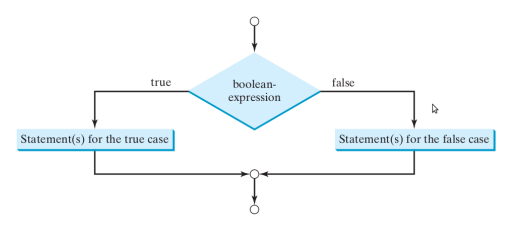
\includegraphics[scale=0.7]{imagenes/ifelse.png}
\caption{if-else}
\end{figure}

\end{frame}

\begin{frame}[fragile]
    \frametitle{Ejemplo de uso en Java}
\begin{scriptsize}
\begin{verbatim}
public class Divisible{
   public static void main(String[] arg){
        int numero = 18;
        if ((numero % 2 == 0) && (numero % 3 ==0))
        {
            System.out.println( "Divisible seis");
        }
        else if (numero % 2 == 0){
             System.out.println("Divisible por dos");
        }
        else if (numero % 3 == 0){
             System.out.println("Divisible por tres");
        }
        else
        {
             System.out.println("No divisible por dos ni por tres");
        }
    }
}
\end{verbatim} 
\end{scriptsize}
\pause
Indica valores de la variable numero para que se cumplan todas las condiciones.
\end{frame}

\begin{frame}[fragile]
\frametitle{El código anterior es equivalente:}
\begin{verbatim}
public class Divisible{
   public static void main(String[] arg){
        int numero = 18;
        if ((numero % 2 == 0) && (numero % 3 ==0))
           System.out.println( "Divisible seis");
        else if (numero % 2 == 0){
           System.out.println("Divisible por dos");
        else if (numero % 3 == 0){
           System.out.println("Divisible por tres");
        else
          System.out.println("No divisible por 
                                 dos ni por tres");
   }
}
\end{verbatim}
\pause
Se omiten las llaves (\{...\}) pues solo hay una sentencia.
\end{frame}



\begin{frame}[fragile]
    \frametitle{¿Y si cambiamos el orden?}
\begin{scriptsize}
\begin{verbatim}
public class Divisible{
   public static void main(String[] arg){
        int numero = 18;
        
        if (numero % 2 == 0 && numero % 3 ==0){
             System.out.println("Divisible por dos");
        }
        else if (numero % 2 == 0)
        {
            System.out.println( "Divisible seis");
        }
        else if (numero % 3 == 0){
             System.out.println("Divisible por tres");
        }
        else
        {
             System.out.println("No divisible por dos ni por tres");
        }
    }
}
\end{verbatim} 
\end{scriptsize}
\end{frame}

\begin{frame}
    \frametitle{Típicos errores}
\begin{itemize}[<+->]

      \item Confundir el operador de asignación con el operador relacional igual:
      \item if (numero \% 2 = 0) 
      \item if (numero \% 2 == 0) 
      \item ¿Cuál es la expresión correcta?
      \item Otro tipo de error es no evaluar correctamente el orden de las condiciones.
      \item Olvidar \{\} en el bloque con mas de una sentencia.
      \item Olvidar el paréntesis en la condición \emph{if x$>$0}
      \item No es error pero es mejor la opción \emph{if (variableBoolean)} que \emph{if (variableBooelan == true)}
      \end{itemize}
      \pause
\end{frame}



\subsection{Iteración}
\begin{frame}
\frametitle{Iteración}
En programación, \emph{Iteración} es la repetición de un proceso dentro de un programa de computadora.\\
Ejemplo: sumar los \emph{n} primeros numeros.
\pause
\begin{block}{}
int suma igual a cero\\
int contador igual a uno\\
mientras que contador sea menor o igual que n\\
\begin{quote}
sumar a suma el valor del contador\\
incrementar el valor del contador\\
\end{quote}
devolver suma
\end{block}
\pause
En java tenemos estructura de control para realizar la iteración: while, do-while, for o switch, 
\end{frame}

\subsection{while y do-while}
\begin{frame}
\frametitle{while y do-while}
\begin{block}{Bucle while}
\begin{itemize}[<+-| alert@+>]
\item while (condicion) \{
\item \ \ \ sentencias;
\item \}
\end{itemize}
\end{block}
\end{frame}


\begin{frame}[fragile]
    \frametitle{Ejemplos}
    \begin{multicols}{2}
\begin{small}
   \begin{verbatim}
public int sumar1(int n){
    int suma = 0;
    int contador =1;
    while (contador <= n){
       suma=suma+contador;
       contador++;
    }
    return suma;
}
\end{verbatim}
\pause
\begin{verbatim}
public int sumar2(int n){
    int suma = 0;
    int contador =1;
    do{
       suma=suma+contador;
       contador++;
    }
    while (contador <= n);
    return suma;
}
\end{verbatim}
%\pause

\end{small}  
\end{multicols}
\pause
\alert{¿Qué ocurre cuando n vale 3,2,1,0?}\\
\pause
\alert{En los casos anteriores ¿cuantas veces se entra en el bucle?}
\end{frame}

\begin{frame}[fragile]
\frametitle{Comprobacion}
\begin{footnotesize}
\begin{multicols}{2}
\begin{tabular}{|c|c|}
\hline
suma & contador\\
\hline
\alert{n}&\alert{3}\\
\hline
0 & 1\\
\hline
1 & 2\\
\hline
3 & 3\\
\hline
6 & 4\\
\hline
\end{tabular}
\begin{tabular}{|c|c|}
\hline
suma & contador\\
\hline
\alert{n}&\alert{2}\\
\hline
0 & 1\\
\hline
1 & 2\\
\hline
3 & 3\\
\hline
\end{tabular}
\begin{tabular}{|c|c|}
\hline
suma & contador\\
\hline
\alert{n}&\alert{1}\\
\hline
0 & 1\\
\hline
1 & 2\\
\hline
\end{tabular}

\begin{tabular}{|c|c|}
\hline
suma & contador\\
\hline
\alert{n}&\alert{0}\\
\hline
0 & 1\\
\hline
\end{tabular}
\begin{verbatim}
public int sumar1(int n){
    int suma = 0;
    int contador =1;
    while (contador <= n){
       suma=suma+contador;
       contador++;
    }
    return suma;
}
\end{verbatim}
\end{multicols}
\end{footnotesize}
\begin{center}
\alert{CONDICION contador $<=n$}
\end{center}
\end{frame}

\begin{frame}[fragile]
\frametitle{Comprobacion}
\begin{footnotesize}
\begin{multicols}{2}
\begin{tabular}{|c|c|}
\hline
suma & contador\\
\hline
\alert{n}&\alert{3}\\
\hline
0 & 1\\
\hline
1 & 2\\
\hline
3 & 3\\
\hline
6 & 4\\
\hline
\end{tabular}
\begin{tabular}{|c|c|}
\hline
suma & contador\\
\hline
\alert{n}&\alert{2}\\
\hline
0 & 1\\
\hline
1 & 2\\
\hline
3 & 3\\
\hline
\end{tabular}
\begin{tabular}{|c|c|}
\hline
suma & contador\\
\hline
\alert{n}&\alert{1}\\
\hline
0 & 1\\
\hline
1 & 2\\
\hline
\end{tabular}

\begin{tabular}{|c|c|}
\hline
suma & contador\\
\hline
\alert{n}&\alert{0}\\
\hline
0 & 1\\
\hline
1 & 2\\
\hline
\end{tabular}
\begin{verbatim}
public int sumar2(int n){
    int suma = 0;
    int contador =1;
    do{
       suma=suma+contador;
       contador++;
    }
    while (contador <= n);
    return suma;
}
\end{verbatim}
\end{multicols}
\end{footnotesize}
\begin{center}
\alert{CONDICION contador $<=n$}
\end{center}
\end{frame}


\begin{frame}[fragile]
\frametitle{do-while}
\begin{verbatim}
public class TestDelDoWhile {
   public static void main (String [ ] Args) {
      int contador = 0 ;
      do {
         System.out.println ("Contando.: " +(contador+1));
         contador += 1;
      } while (contador<10);
   }   
}
\end{verbatim}
¿Cuál es la salida del programa?
\end{frame}


\begin{frame}
\frametitle{Diferencia while, do-while}
\begin{itemize}[<+->]
\item La unica diferencia entre \emph{while} y \emph{do-while} es que la sentencia \alert{do-while} se ejecuta siempre, al menos, una vez incluso aunque la expresion condicional sea falsa.
\item En \alert{while} si la condicion es falsa la primera vez, la sentencia no se ejecuta nunca.
\item En la practica \alert{do-while} es menos comun que \alert{while}.
\end{itemize}
\pause
\end{frame}



\subsection{Bucle for}
\begin{frame}
\frametitle{for}
\begin{block}{definicion}
\begin{itemize}[<+->]
\item \emph{for }(inicializacion; condicion; paso)
\item \{
\item \ \ \ sentencias
\item \}
\end{itemize}
\end{block}
\pause
\begin{block}{Ejemplo:}
\begin{itemize}[<+->]
\item int suma=0; 
\item for (int i=1; i$<$=n; i++ ) \{
\item \  \ \ suma += i;
\item \}
\end{itemize}
Se puede omitir el bloque, pués solo hay una sentencia.
\pause
\end{block}

\end{frame}

\begin{frame}[fragile]
\frametitle{break}
\framesubtitle{¿Qué hace este código?}

\begin{footnotesize}
\begin{verbatim}
//buscar los n primeros múltiplos de un número
      int numero = 1100120;
      int n = 0;
      int contadorMultiplos = 0;
      int contadorGeneral   = 1;
      while (contadorGeneral < numero) {
          if ( numero  % contadorGeneral == 0) {
              System.out.println("Divisor " +
                       contadorGeneral);
              contadorMultiplos++;
          }
          if (contadorMultiplos == 10) {
                break;
          }
          contadorGeneral++;
      }                     
\end{verbatim}
\pause
La sentencia \emph{break} sale del bucle sin ejecutar el resto de las sentencias del bucle
\end{footnotesize}
\end{frame}

\begin{frame}[fragile]
\frametitle{continue}
\framesubtitle{¿Qué hace este código?}
\begin{verbatim}
public static int numeroConsonantes(String palabra){
    int contador=0;
    for (int i=0; i<palabra.length(); i++){
        String letra = palabra.substring(i,i+1);
        if (letra.contains("a") || letra.contains("e") ||
            letra.contains("i") || letra.contains("o") ||
            letra.contains("u") || letra.contains(" ")){
                  continue;
        }
        contador++;
    }
    return contador;
}
\end{verbatim}
\pause
\alert{La sentencia \emph{continue} detiene la ejecución del bucle y vuelve al principio de éste.}
\end{frame}

\subsection{switch}
\begin{frame}
\frametitle{switch}
\begin{itemize}[<+->]
\item Es un operador que permite decidir entre diferentes opciones.
\item Se inicia con la palabra clave \emph{swtich}
\item En funcion del parametro que se le pase se seleccionara una opcion u otra, definidas junto a la palabra clave \emph{case}
\item En caso que la condicion no coincida con ninguna opcion se ejecuta la sentencia que acompaña a la palabra clave \emph{default}
\item Se usa la palabra clave \emph{break} para finalizar cada \emph{case}
\item Es similar a la usada en \emph{lenguaje C}
\end{itemize}
\pause
\end{frame}

\begin{frame}[fragile]
\frametitle{switch}
\begin{multicols}{2}
\begin{verbatim}
switch (condicion){
   case valor1:
      sentencias;
      break;
   case valor2:
      sentencias;
      break;
      
   ...............
   
   default:
      sentencias
}   
\end{verbatim}
\pause
\begin{verbatim}
String dia;
switch (d){
   case 1:
      dia="Lunes";
      break;
   case 2:
      dia="Martes";
      break;
      
   ...............
   
   default:
      dia="Domingo";
}   
\end{verbatim}
\end{multicols}
\pause
¿Cuántos \emph{case} debe haber en el último ejemplo?
\end{frame}

\subsection{Bucles anidados}
\begin{frame}[fragile]
\frametitle{Bucles anidados}
\begin{verbatim}
for (int i=0; i<3;i++){
    for (int j=0; j<3;j++){
        System.out.println(i*j);
    }
}
\end{verbatim}
¿Cuál es la salida de este código?
\end{frame}


\section{Miscelanea}
\subsection{if-else}
\begin{frame}[fragile]
\frametitle{if-else}
\begin{itemize}[<+-|alert@+>]
\item Podemos definir la estructura de control \emph{if-else} de la siguiente forma:
\item \emph{condicion ? valorCierto : valorFalso}
\item Ejemplo:
\item String mensaje = (numero \% 2 ==0) ? ''Es par" : ''Es impar";
\end{itemize}
\pause
\end{frame}

\subsection{Concatenar cadenas}
\begin{frame}[fragile]
\frametitle{Concatenar cadenas}
\begin{itemize}[<+-|alert@+>]
\item Se trata de unir dos o mas cadenas.
\item Usamos el operador \emph{+}
\item Ejemplo:
\item String mensaje1 ="hola"; String mesanje2="Ruben";
\item String mensajeFinal = mensaje1+ '' ''+mensaje2;
\item ¿Cual es el mensaje final?
\item También se pueden usar otros tipos además de \emph{String}
\item int numero=66666666;
\item String mensajeFinal = "Telefono de+ '' ''+mensaje2+'' ''+numero;
\item En este caso hay una conversión de tipos \emph{(casting)} a tipo \emph{String}
\end{itemize}
\pause
\end{frame}

\subsection{Argumentos en la linea de comandos}
\begin{frame}[fragile]
\frametitle{Argumentos en la linea de comandos}
\begin{itemize}[<+-|alert@+>]
\item Son los parametros que el programa recibe desde la linea de comandos.
\item Ejemplo cuando ejecutamos en GNU/Linux \emph{ls -la}
\item El comando es \emph{ls} y los parametros son \emph{la}
\item En caso de java: \emph{java Programa argumento1 argumento2 \dots}
\item Se acceden a traves de String[ ]
\item \emph{public static void main(String[ ] args)}
\item Ejemplo:
\end{itemize}
\pause
\begin{verbatim}
public class Argumentos{
    public static void main(String[] args){
        System.out.println("Argumento 1: "+args[0]);
        System.out.println("Argumento 2: "+args[1]);
    }
}
\end{verbatim}
\begin{footnotesize}
\pause
\begin{enumerate}[<+->]
\item ¿Si se ejecuta java Argumentos uno dos? ¿Cuál es la salida?
\item ¿Si se ejecuta java Argumentos uno ? ¿Cuál es la salida?
\item ¿Si se ejecuta java Argumentos uno dos tres? ¿Cuál es la salida?
\end{enumerate}
\end{footnotesize}
\pause
\end{frame}


\subsection{Formateando salida}
\begin{frame}[fragile]
\frametitle{printf}
\begin{itemize}[<+-|alert@+>]
\item \emph{printf} nos permite dar formato a los datos que se imprimen en pantalla.
\item Ejemplo para mostrar el número \emph{12.3698} con dos decimales usamos:
\item \emph{System.out.printf(''\%.2f \%n'', 12.3698);}
\item El primer \% indica que en esa posición se va a escribir un valor. El valor a escribir se encuentra a continuación de las comillas. 
\item .2 indica el número de decimales
\item La \emph{f} indica que el número es de tipo float o double.
\item \%n indica un salto de línea. Equivale a $\backslash n$. Con printf podemos usar ambos para hacer un salto de línea.
\item La salida por pantalla es 12,37
\end{itemize}
\pause
\end{frame}

\begin{frame}
\frametitle{Especificadores para printf}
\begin{tabular}{ccc}
\hline
Especificador & Salida & Ejemplo \\
\hline
\%b &Valor booleano & true o false\\
\%c & un caracter&'d' \\
\%d & un número entero & 200\\
\%f & un número en coma flotante& 45.4689\\
\%e & un número en notación científica & 4.556000e+01\\
\%s & un string&''hola mundo'' \\
\end{tabular}
\pause
\begin{figure}
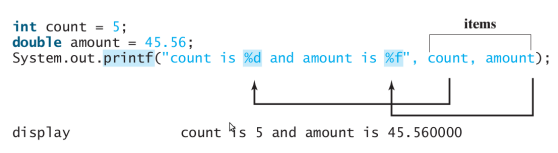
\includegraphics[scale=0.6]{imagenes/formateo.png}
\caption{Ejemplo de printf}
\end{figure}
\end{frame}

\begin{frame}[fragile]
\frametitle{Ejemplos de printf}
\framesubtitle{¿Cuál es la salida de printf?}
\begin{itemize}[<+->]
\item double n = 1.25036; System.out.printf("\%.3f \%n", n);
\item \alert{1,250}
\item double n = 1.25036; System.out.printf("\%+.3f \%n", n);
\item \alert{+1,250}
\item int x = 10; System.out.printf("\%d \%n", x);
\item \alert{10}
\item double n = 1.25036; int x = 10; System.out.printf("n = \%.2f x = \%d \%n", n, x);.
\item \alert{n = 1,25 x = 10}
\item double n = 1.25036; System.out.printf("\%+10.2f \%n", n);
\item \alert{bbbbb+1.25} Donde b representa un espacio en blanco.
\item double n = 1.25036; System.out.printf("\%+010.2f \%n", n);
\item \alert{b+000001.25}
\end{itemize}
\pause
\end{frame}

\begin{frame}[fragile]
\frametitle{Ejercicios de printf}
\framesubtitle{¿Cómo debemos formatear con printf?}
\begin{itemize}[<+->]
\item Mostrar el número 1.22 en un ancho de campo de 10 caracteres y con dos decimales.
\item \alert{double precio = 1.22; System.out.printf(''\%10.2f'', precio);}
\item Mostrar la cadena ''Total:''con un ancho de 10 caracteres y alineada a la izquierda
\item \alert{System.out.printf(''\%-10s'', ''Total:'');} (Por defecto se alinea a la derecha).
\item System.out.printf(''\%8d\%8s\%8.1f$\backslash n$'', 1234, ''Java'', 5.6);
\item System.out.printf(''\%-8d\%-8s\%-8.1f $\backslash n$'', 1234, ''Java'', 5.6);
\item Muestra:
\end{itemize}
\pause
\begin{figure}
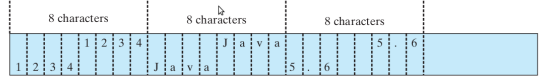
\includegraphics[scale=0.6]{imagenes/display.png}
\end{figure}
\end{frame}


\begin{frame}
\frametitle{Preguntas} 
\begin{figure}

\includegraphics[scale=0.9]{imagenes/dudas.png} 
\caption{¿dudas?}
\end{figure} 
\end{frame}



\end{document}

